\begin{frame}{Data Explanation}
\begin{itemize}
 \item 1514 MD Anderson patients who had brainmets from breast cancer
 \item 90 covariates
 \begin{itemize}
  \item Missingness from 0 to 65\%
 \end{itemize}

\end{itemize}
\begin{table}[!ht]
\centering
\begin{tabular}{|c|c|}
\hline
Type                                                                            & Example                                                                       \\ \hline
Subject data                                                                    & Age range, race, date of birth                                                \\ \hline
Cancer data                                                                     & TNM staging, type, receptor status                                            \\ \hline
\begin{tabular}[c]{@{}c@{}}Pre brain mets\\ data\end{tabular}                   & Treatment types                                                               \\ \hline
\begin{tabular}[c]{@{}c@{}}Post brain mets\\ clinical observations\end{tabular} & Seizures, headache, nasuea                                                    \\ \hline
\begin{tabular}[c]{@{}c@{}}Post brain mets\\ data\end{tabular}                  & \begin{tabular}[c]{@{}c@{}}Treatment type, \\ type of brain mets\end{tabular} \\ \hline
Survival data                                                                   & Survival time after brain mets, censoring indicator                           \\ \hline
\end{tabular}
\caption{Data Categories and Examples}
\label{table:cats}
\end{table}

\end{frame}

\begin{frame}{Important Covariates}
 \begin{table}[ !ht]
\centering
\adjustbox{max height=\dimexpr\textheight-5.5cm\relax,
           max width=\textwidth}{
\begin{tabular}{|c|c|c|}
\hline
Name        & \begin{tabular}[c]{@{}c@{}}Percent \\ Missing\end{tabular} & Meaning                                                                                                                                             \\ \hline
hrher2      & 5                                                        & \begin{tabular}[c]{@{}c@{}}Categorical variable: The hormonal receptor and \\ HER2 receptor status of the subject\end{tabular}                      \\ \hline
agebrainmet & 0                                                          & Indicator: Age greater or less than 60 at time of brain mets                                                                                        \\ \hline
timedx      & 1                                                         & \begin{tabular}[c]{@{}c@{}}Indicator: Time (years) from breast cancer diagnosis to brain\\ mets diagnosis greater or less than 6 years\end{tabular} \\ \hline
site5       & 1                                                        & Indicator: First metastasis was to brain                                                                                                            \\ \hline
race2       & 0                                                          & Categorical: White, Black, Hispanic, other                                                                                                          \\ \hline
priorn      & 0                                                          & \begin{tabular}[c]{@{}c@{}}Indicator: Number of prior treatments in metastatic setting \\ before brain mets\end{tabular}                            \\ \hline
braintype   & 4                                                        & Categorical: Single, multiple, Leptomeningeal disease                                                                                               \\ \hline
controlled  & 12                                                        & Indicator: Extracranial progression of brain mets                                                                                                   \\ \hline
capeothno   & 18                                                        & \begin{tabular}[c]{@{}c@{}}Indicator: Capecitabine, other, or no chemotheraputic\\ treatment. Treatment variable 1\end{tabular}                     \\ \hline
lapatrasno  & 18                                                        & \begin{tabular}[c]{@{}c@{}}Indicator: Lapatinib, Trastuzumab, or no HER2 treatment.\\ Treatment variable 2\end{tabular}                             \\ \hline
os          & 0                                                          & Overall survival (months)                                                                                                                           \\ \hline
dead        & 0                                                          & Indicator: death indicator                                                                                                                          \\ \hline
her2        & 10                                                        & Indicator: HER2 receptor status                                                                                                                     \\ \hline
\end{tabular}
}
\caption{Table of important covariates to be used in the analysis}
\label{table:importantvars}

\end{table}
\end{frame}

\begin{frame}{Visualization of Missingness}
 \begin{figure}[h!]
  \centering
    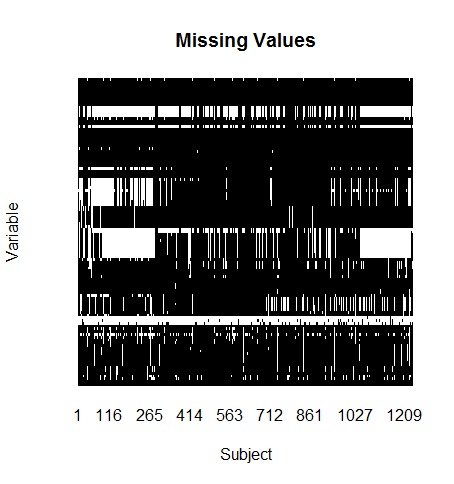
\includegraphics[width=0.8\textwidth]{missingvalues_plot.png}
  \caption{Visualization of missingness in the cancer dataset}
\label{fig:missingplot}

\end{figure}
\end{frame}

\begin{frame}{Imputation}
 \begin{itemize}
  \item MAR assumption seems reasonable
  \item FCS over JM due to nature of data
  \item Need to set up models and predictors
  \item Check for convergence and validity
 \end{itemize}

\end{frame}

\begin{frame}{Setting up the model}
Issues
\begin{itemize}
 \item Many categorical variables 
 \item Collinearity between predictors
 \item Variables with poor influx/outflux \cite{VanBuuren2012}
 \item How many iterations and imputations to draw?
\end{itemize}

 
\end{frame}


\begin{frame}{Convergence}
 
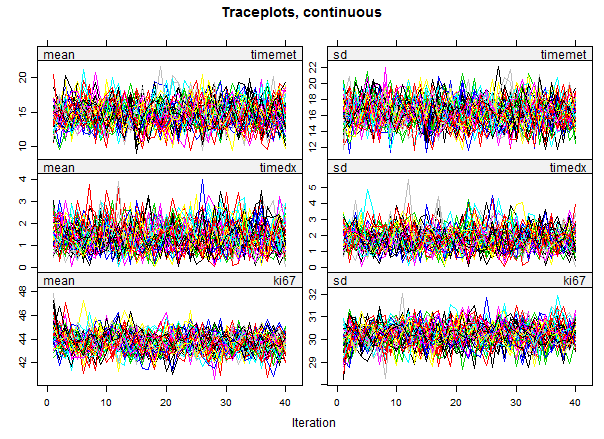
\includegraphics[width=.5\textwidth]{traceplots1}%
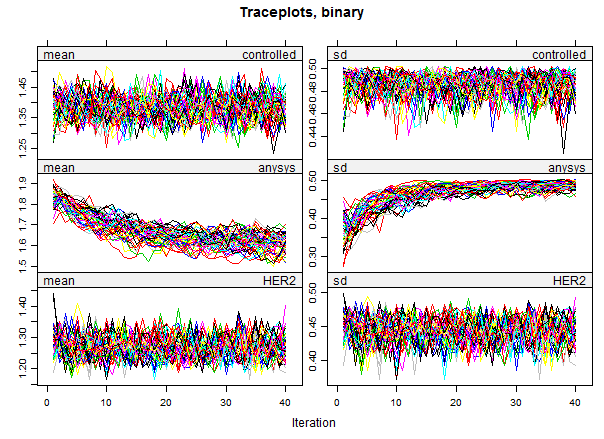
\includegraphics[width=.5\textwidth]{traceplots2} 

\note{On convergence, the different streams should be freely intermingled with one another,
without showing any definite trends. Convergence is diagnosed when the variance between different 
sequences is no larger than the variance within each individual sequence.}
\end{frame}

\begin{frame}{Validity}
 \begin{itemize}
  \item Lots of tools for continous imputations
  \item not many for categorical
  \begin{itemize}
   \item Solution: look at tables to verify validity
  \end{itemize}

 \end{itemize}

\end{frame}

\begin{frame}{Validity Checks}
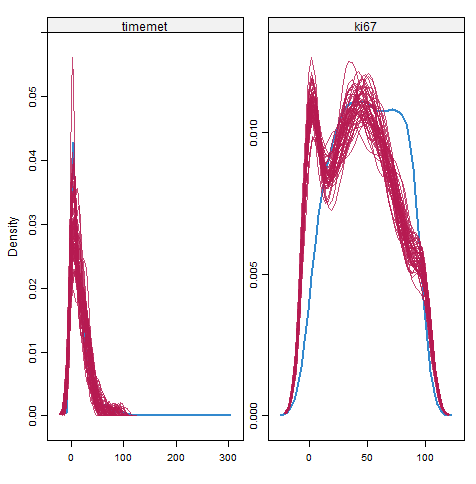
\includegraphics[width=.5\textwidth]{cont_densplot}%
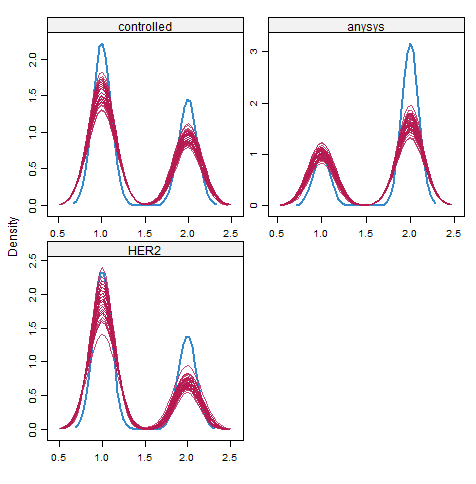
\includegraphics[width=.5\textwidth]{discrete_densplot} 
\end{frame}

\begin{frame}{Validity Checks}
 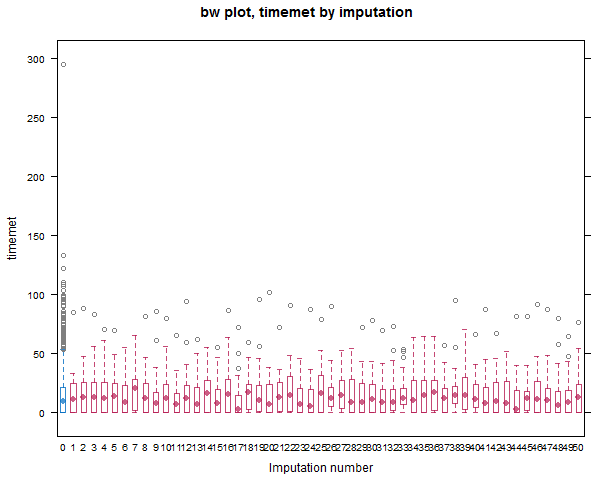
\includegraphics[width=.5\textwidth]{bw_timemet}%
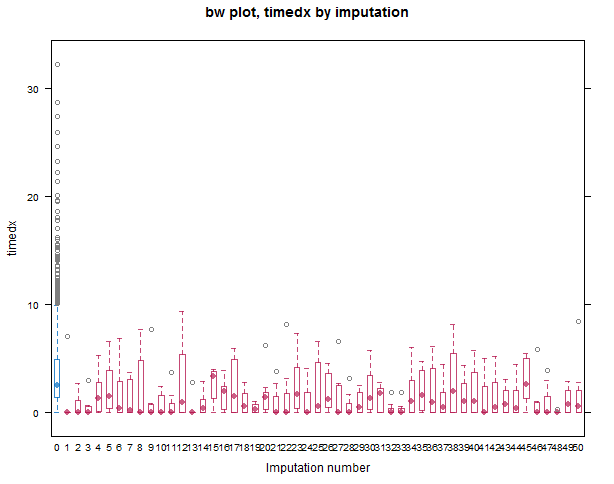
\includegraphics[width=.5\textwidth]{bw_timedx} 
\end{frame}

\begin{frame}{Tabluar Checks}
 %figure this out
 %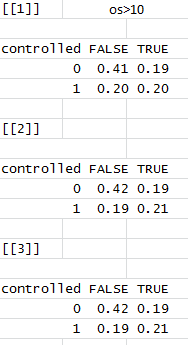
\includegraphics[width=.5\textwidth,height=.5\textwidth]{oscontrol_table}%
%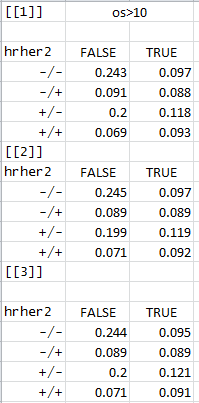
\includegraphics[width=.5\textwidth]{oshrher2_table} 
\end{frame}

\begin{frame}{MI data Breakdown}
\begin{table}[!ht]
\adjustbox{max height=\dimexpr\textheight-5.5cm\relax,
           max width=\textwidth}{
\centering
\begin{tabular}{|r|c|c|c|c|}
\hline
\multicolumn{1}{|l|}{}                            & \begin{tabular}[c]{@{}c@{}}Sys therapy \\ available case\end{tabular} & \begin{tabular}[c]{@{}c@{}}Sys therapy \\ MI\end{tabular} & \begin{tabular}[c]{@{}c@{}}No Sys therapy \\ available case\end{tabular} & \begin{tabular}[c]{@{}c@{}}No Sys therapy \\ MI\end{tabular} \\ \hline
\multicolumn{1}{|l|}{Age (mean,sd)}               & 51.4(10.8)                                                            & 51.2(10.9)                                                & 52.7(11.9)                                                               & 52.9(11.4)                                                   \\ \hline
\multicolumn{1}{|l|}{Breast Cancer subtype}       &                                                                       &                                                           &                                                                          &                                                              \\ \hline
HR+/HER2-                                         & 27\%                                                                  & 31\%                                                      & 28\%                                                                     & 33\%                                                         \\ \hline
HR+/HER2+                                         & 19\%                                                                  & 18\%                                                      & 12\%                                                                     & 13\%                                                         \\ \hline
HR-/HER2+                                         & 22\%                                                                  & 20\%                                                      & 15\%                                                                     & 12\%                                                         \\ \hline
Triple negative                                   & 32\%                                                                  & 32\%                                                      & 45\%                                                                     & 42\%                                                         \\ \hline
\multicolumn{1}{|l|}{Prior therapies for stage 4} & 1(0-3)                                                                & 2(0-4)                                                    & 2(0-4)                                                                   & 2(0-4)                                                       \\ \hline
\multicolumn{1}{|l|}{Single brain lesion}         & 25\%                                                                  & 23\%                                                      & 23\%                                                                     & 20\%                                                         \\ \hline
\multicolumn{1}{|l|}{Controlled extra-cranial}    & 40\%                                                                  & 40\%                                                      & 35\%                                                                     & 36\%                                                         \\ \hline
\multicolumn{1}{|l|}{ECOG 0-1}                    & 84\%                                                                  & 70\%                                                      & 53\%                                                                     & 40\%                                                         \\ \hline
\multicolumn{1}{|l|}{Local Therapy}               &                                                                       &                                                           &                                                                          &                                                              \\ \hline
Resection Alone                                   & 5\%                                                                   & 5\%                                                       & 9\%                                                                      & 7\%                                                          \\ \hline
SBRT alone                                        & 13\%                                                                  & 12\%                                                      & 9\%                                                                      & 8\%                                                          \\ \hline
WBRT                                              & 60\%                                                                  & 59\%                                                      & 52\%                                                                     & 53\%                                                         \\ \hline
Resection/SBRT+WBRT                               & 12\%                                                                  & 14\%                                                      & 10\%                                                                     & 8\%                                                          \\ \hline
no local therapy                                  & 10\%                                                                  & 10\%                                                      & 20\%                                                                     & 23\%                                                         \\ \hline
\end{tabular}
}
\caption{Characteristics of available case data versus MI data}
\label{table:chartab}
\end{table}
 
\end{frame}

\begin{frame}{Kaplan-Meier in MI}
 \begin{itemize}
  \item Noninformative censoring reasonable
  \item Pooled by Rubin's Rules on Complimentary log-log
 \end{itemize}
 \begin{figure}[h!]
  \centering
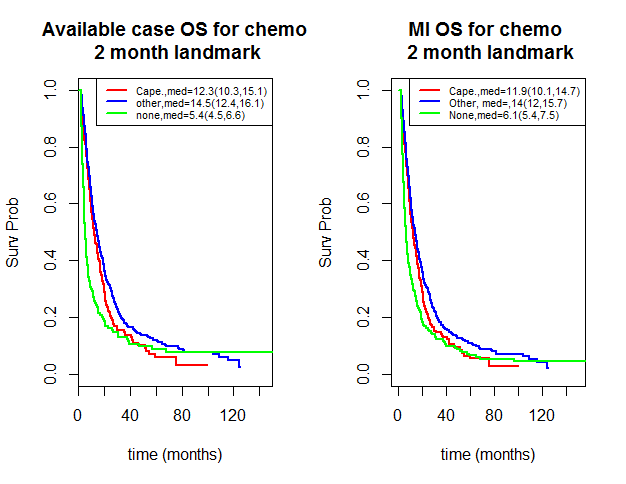
\includegraphics[width=.8\textwidth]{cape_km}
\end{figure}
\end{frame}

\begin{frame}{Kaplan-Meier in MI}
 \begin{figure}[h!]
  \centering
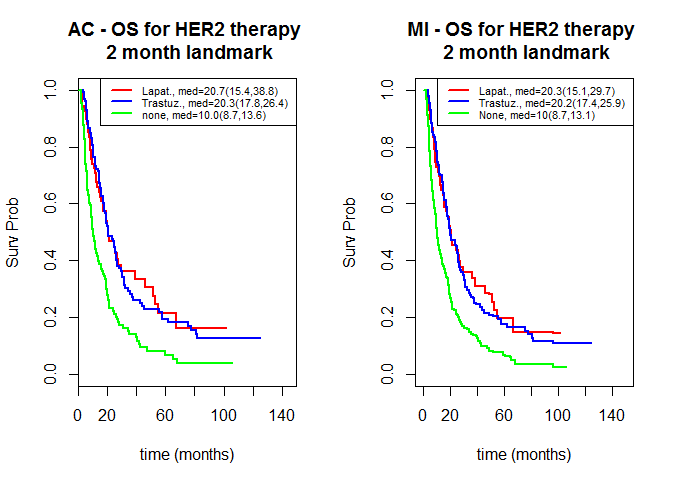
\includegraphics[width=.8\textwidth]{lapat_km}
\end{figure}
 
\end{frame}

\begin{frame}{Log Rank Test}
\begin{table}[]
\centering
\begin{tabular}{|l|c|c|}
\hline
                & \multicolumn{2}{c|}{Chemo}                         \\ \hline
                & \multicolumn{1}{l|}{AC} & \multicolumn{1}{l|}{MI} \\ \hline
cape/other/none & \textless.0001          & \textless.0001          \\ \hline
cape/other      & 0.0321                  & 0.033                   \\ \hline
cape/none       & 0.00039                 & .0016                   \\ \hline
other/none      & \textless.0001          & \textless.0001          \\ \hline
\end{tabular}
\end{table}

\begin{table}[]
\centering
\begin{tabular}{|l|c|c|}
\hline
                   & \multicolumn{2}{c|}{HER2}                         \\ \hline
                   & \multicolumn{1}{l|}{AC} & \multicolumn{1}{l|}{MI} \\ \hline
Lapat/Traztuz/none & \textless.0001          & \textless.0001          \\ \hline
Lapat/Trastuz      & .87                     & .81                     \\ \hline
Lapta/none         & .00017                  & .00018                  \\ \hline
Trastuz/none       & \textless.0001          & \textless.0001          \\ \hline
\end{tabular}
\end{table}
\end{frame}
